\documentclass{article}

\usepackage{graphicx}
\usepackage[hidelinks]{hyperref}
\usepackage[a4paper, total={6in, 8in}]{geometry}
\usepackage[slovak]{babel}
\usepackage{caption}
\usepackage{subcaption}
\usepackage{listings}

\graphicspath{./include/}

\renewcommand{\figurename}{Obr.}
\renewcommand{\contentsname}{Obsah}

\begin{document}

\begin{titlepage}
	\null\vfill

	\begin{center}
		{\Huge Magnetická levitácia }
		\vskip 2cm

		{\Large Cvičenie č. 8}
		\vskip 0.5cm

		{\large Spojité procesy}
	\end{center}

	\vfill
	\vfill

	\begin{flushright}
		Filip Lobpreis \\
		Matúš Machata \\
		\small\today\\
	\end{flushright}
	\hfill
\end{titlepage}

\thispagestyle{empty}
\clearpage

\tableofcontents
\thispagestyle{empty}
\clearpage

\section{Zadanie}
\label{sec:zadanie}

\begin{figure}[!htbp]
	\begin{center}
		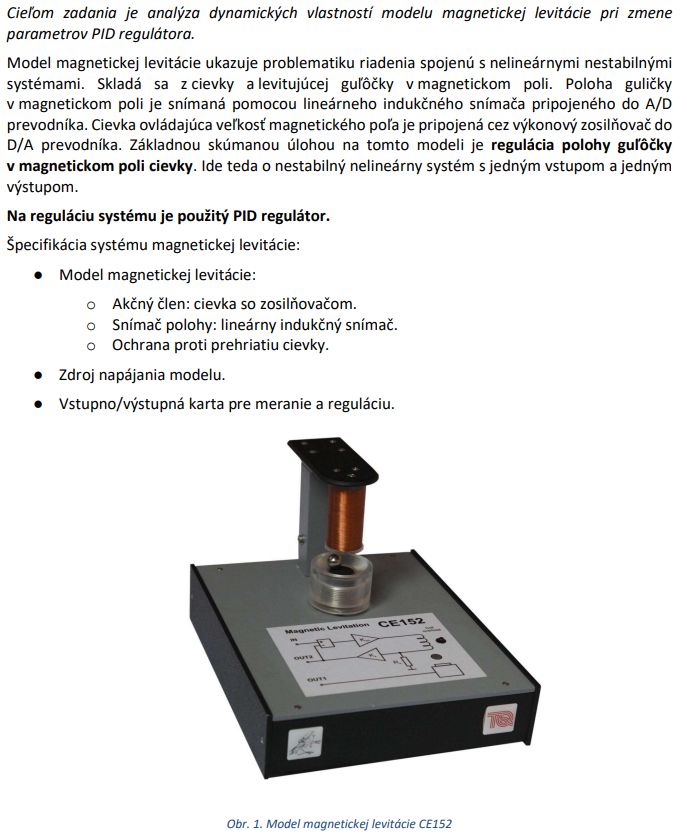
\includegraphics[width=0.95\textwidth]{include/zadanie.png}
	\end{center}
	\caption{Zadanie č. 8 z~predmetu Spojité procesy.}
	\label{fig:zadanie}
\end{figure}

\pagenumbering{arabic}
\clearpage

\section{Merania}
\label{sec:merania}

Ôsme zadanie z~predmetu spojité procesy sa zaoberá skúmaním vplyvu zmien koeficientov PID regulátora
na~ovládanie magnetickej levitácia. V~tomto zadaní budeme postupne meniť PID regulátor a~jeho \textbf{Proporcionálnu},
\textbf{Integračnú} a~\textbf{Derivačnú} zložku. Na~obrázku Obr.~\ref{fig:schema} vidíme model magnetickej levitácia,
ktorý sme použili pri~meraniach. Jednotlive parametre regulatora budeme menit v~rozsahu $\pm20\%$.

\begin{figure}[!htbp]
	\begin{center}
		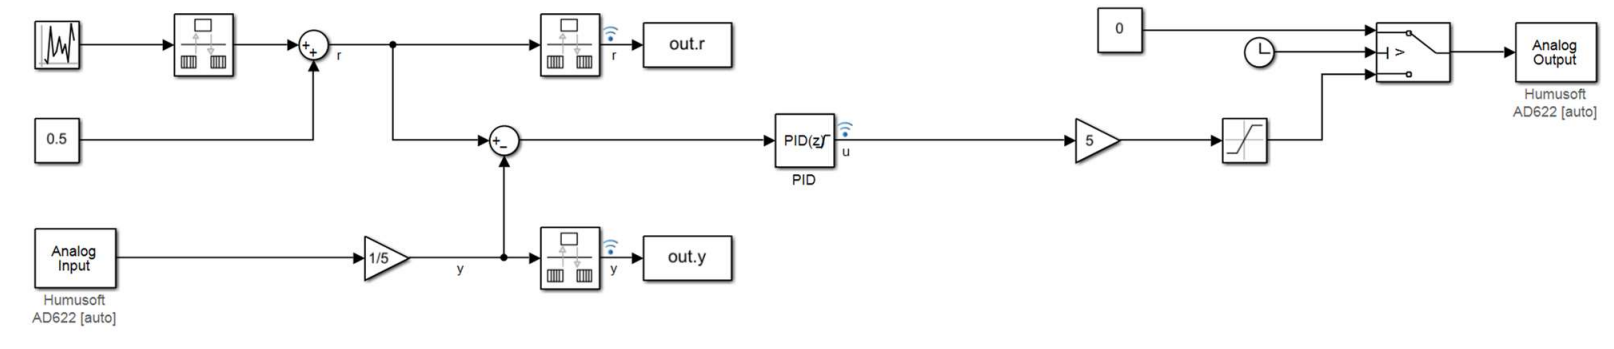
\includegraphics[width=0.95\textwidth]{include/schema.png}
	\end{center}
	\caption{Schéma pre~model magnetickej levitácie.}
	\label{fig:schema}
\end{figure}

\begin{table}[!htbp]
	\caption{Koeficienty PID regulatora}
	\label{tab:t0}
	\begin{center}
		\begin{tabular}[c]{|l|l|}
			\hline

			P & 1 \\
			I & 4 \\
			D & 0.016 \\
			\hline
		\end{tabular}
	\end{center}
\end{table}

\begin{figure}[!htbp]
	\begin{center}
		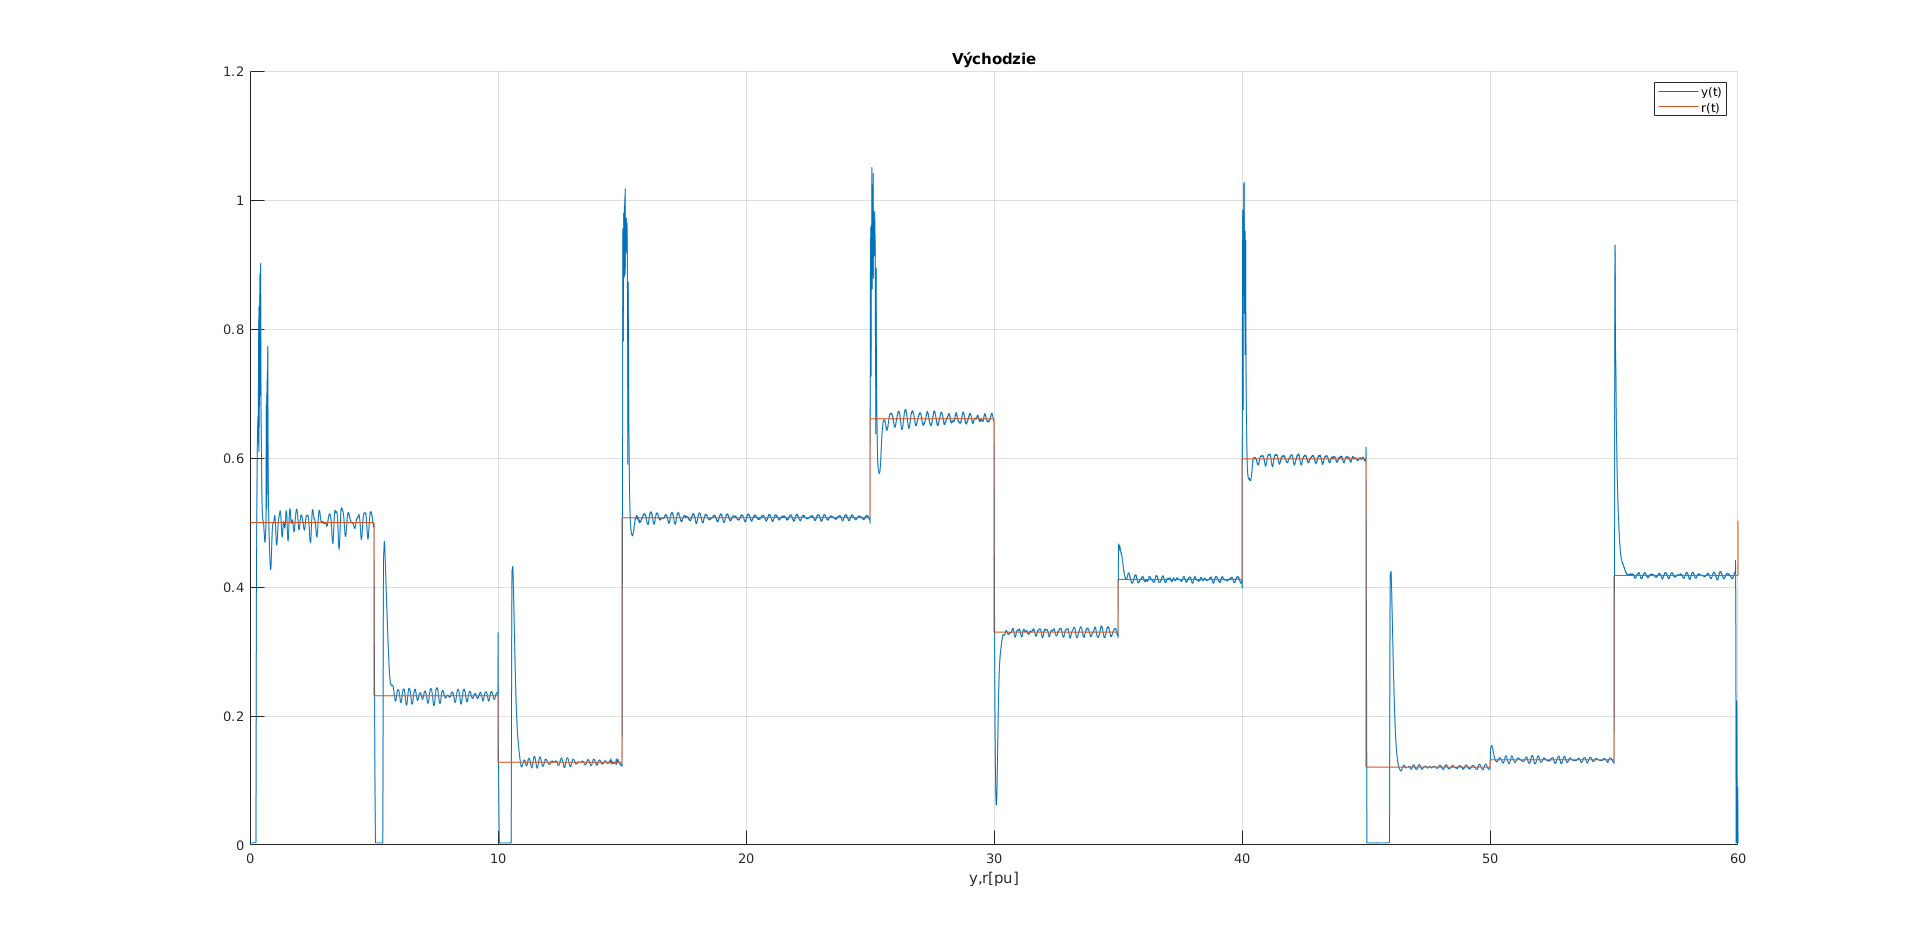
\includegraphics[width=0.95\textwidth]{include/m1.png}
	\end{center}
	\caption{Zakladne hodnoty PID regulatora.}
	\label{fig:m1}
\end{figure}

Obrazok Obr.~\ref{fig:m1} zobrazuje kmitavý tlmený proces s~preregulovaním. Mozeme vidiet, ze ci vyssie mal
regulator udrzat kovovu gulicku, tym viac bol system rozkmitany. Pri~prvych petnastich sekundach merania
magneticke pole nedokazalo dostatocne stabilizovat gulicku a~nastaval velky rozkmit v~ustalenej hodnote.

\clearpage

\subsection{Meranie 1}
\label{sec:meranie1}

\begin{table}[!htbp]
	\caption{Koeficienty PID regulatora}
	\label{tab:t1}
	\begin{center}
		\begin{tabular}[c]{|l|l|}
			\hline
			P & 1.2 \\
			I & 4 \\
			D & 0.016 \\
			\hline
		\end{tabular}
	\end{center}
\end{table}

\begin{figure}[!htbp]
	\begin{center}
		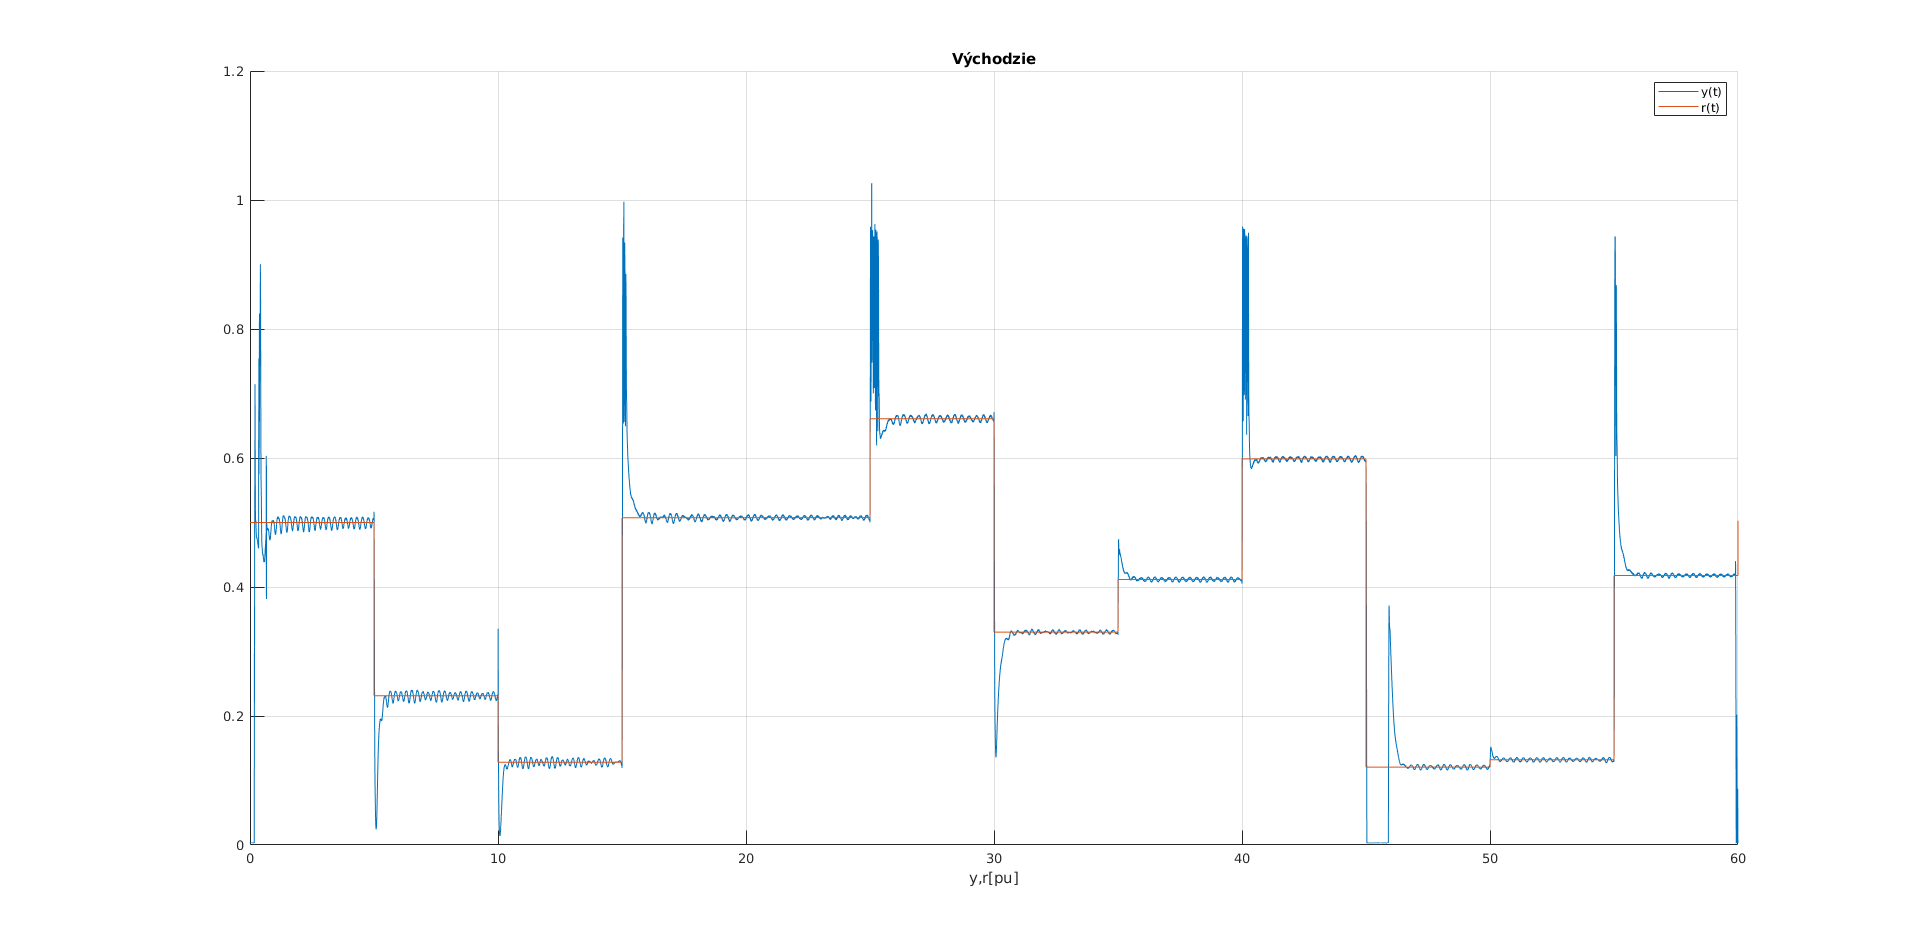
\includegraphics[width=0.8\textwidth]{./include/m2.png}
	\end{center}
	\caption{Graf prveho merania.}
	\label{fig:meranie1}
\end{figure}

V~druhom merani sme zvysili \textbf{propoccionalnu} zlozku regulatora o~20\%. Vysledok je viditelny
na~obrazku Obr.~\ref{fig:meranie1}. Taktiez ako v~predchadzajucom merani bolo prvych petnast sekund
merania rozkmitanych. V~dalsich skokoch vidime vacsi ucinok derivacnej zlozky. Toto sposobilo zvysenie
uz spomenutej proporcionalnej zlozky.

\clearpage

\subsection{Meranie 2}
\label{sec:meranie2}

\begin{table}[!htbp]
	\caption{Koeficienty PID regulatora}
	\label{tab:t2}
	\begin{center}
		\begin{tabular}[c]{|l|l|}
			\hline
			P & 0.8 \\
			I & 4 \\
			D & 0.016 \\
			\hline
		\end{tabular}
	\end{center}
\end{table}

\begin{figure}[!htbp]
	\begin{center}
		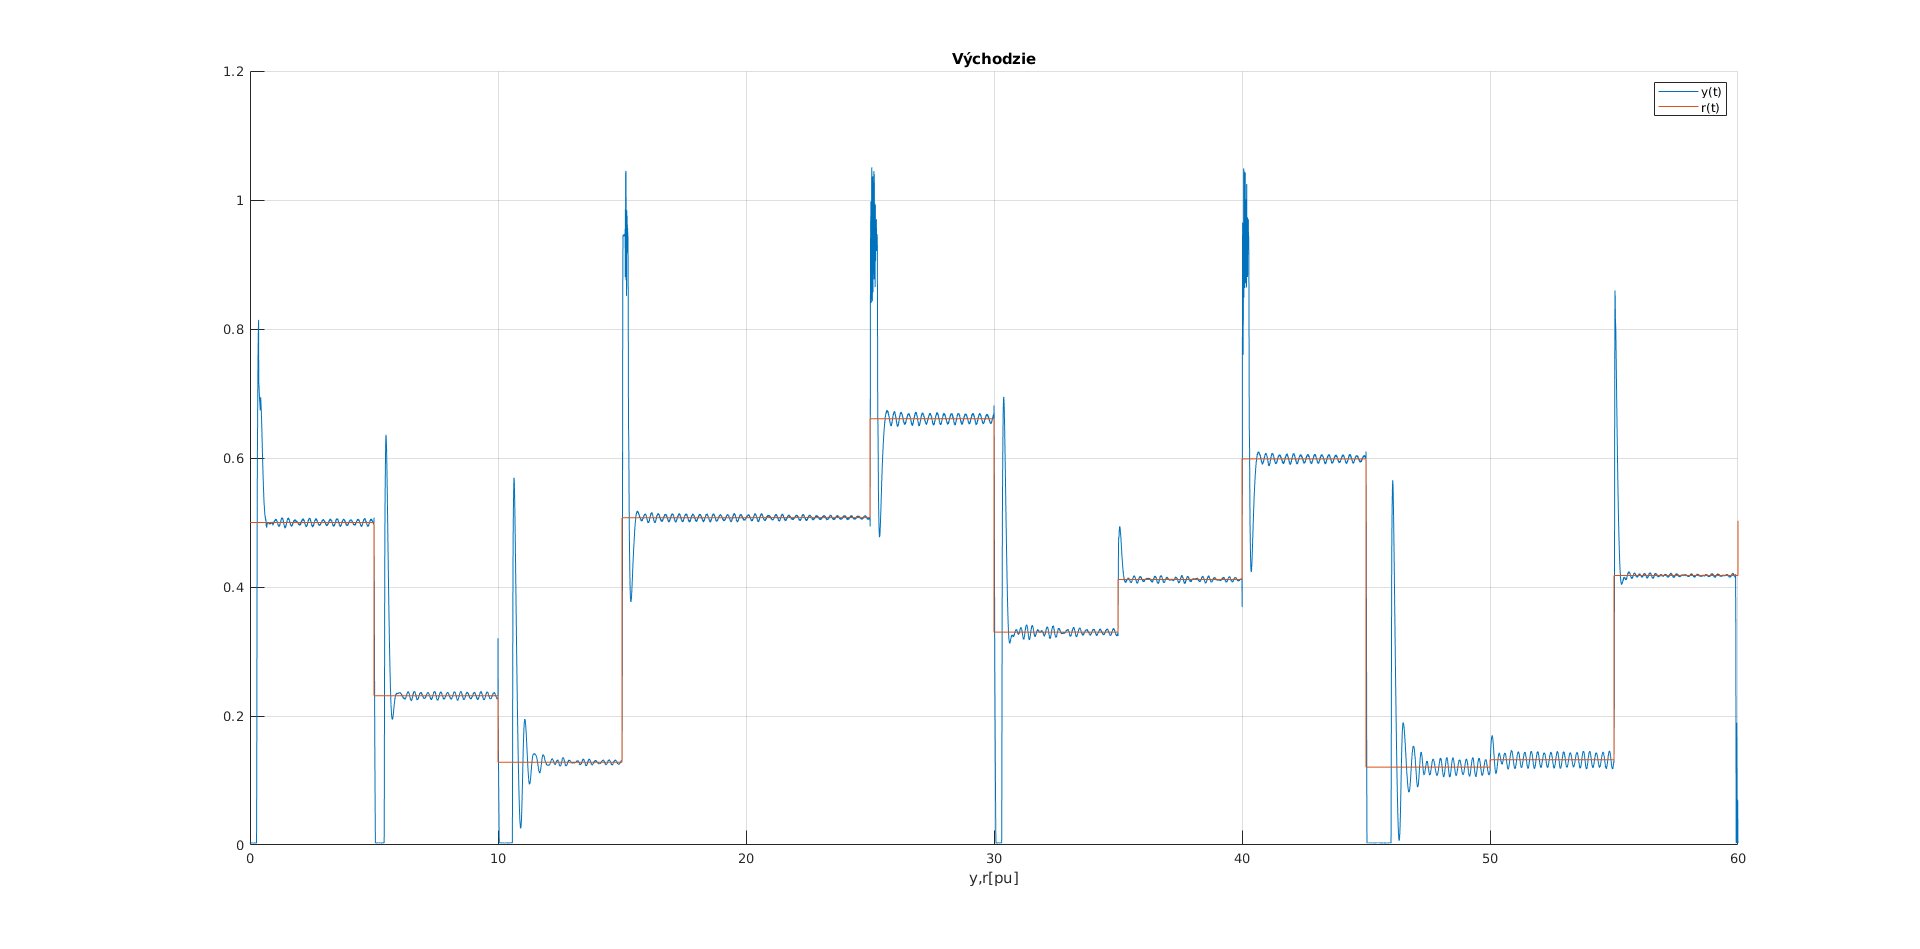
\includegraphics[width=0.8\textwidth]{./include/m3.png}
	\end{center}
	\caption{Graf druheho merania.}
	\label{fig:meranie2}
\end{figure}

V~tretom merani sme zmensili \textbf{propoccionalnu} zlozku regulatora o~20\%. Vysledok je viditelny
na~obrazku Obr.~\ref{fig:meranie2}. Taktiez ako v~predchadzajucom merani bolo prvych petnast sekund
merania rozkmitanych s tym rozdielom, ze zmensenie proporcionalnej zlozky malo za dosledok mensiu
stabilitu systemu pri zmenseni ziadanej hodnoty.

\clearpage

\subsection{Meranie 3}
\label{sec:meranie3}

\begin{table}[!htbp]
	\caption{Koeficienty PID regulatora}
	\label{tab:t3}
	\begin{center}
		\begin{tabular}[c]{|l|l|}
			\hline
			P & 1 \\
			I & 4.8 \\
			D & 0.016 \\
			\hline
		\end{tabular}
	\end{center}
\end{table}

\begin{figure}[!htbp]
	\begin{center}
		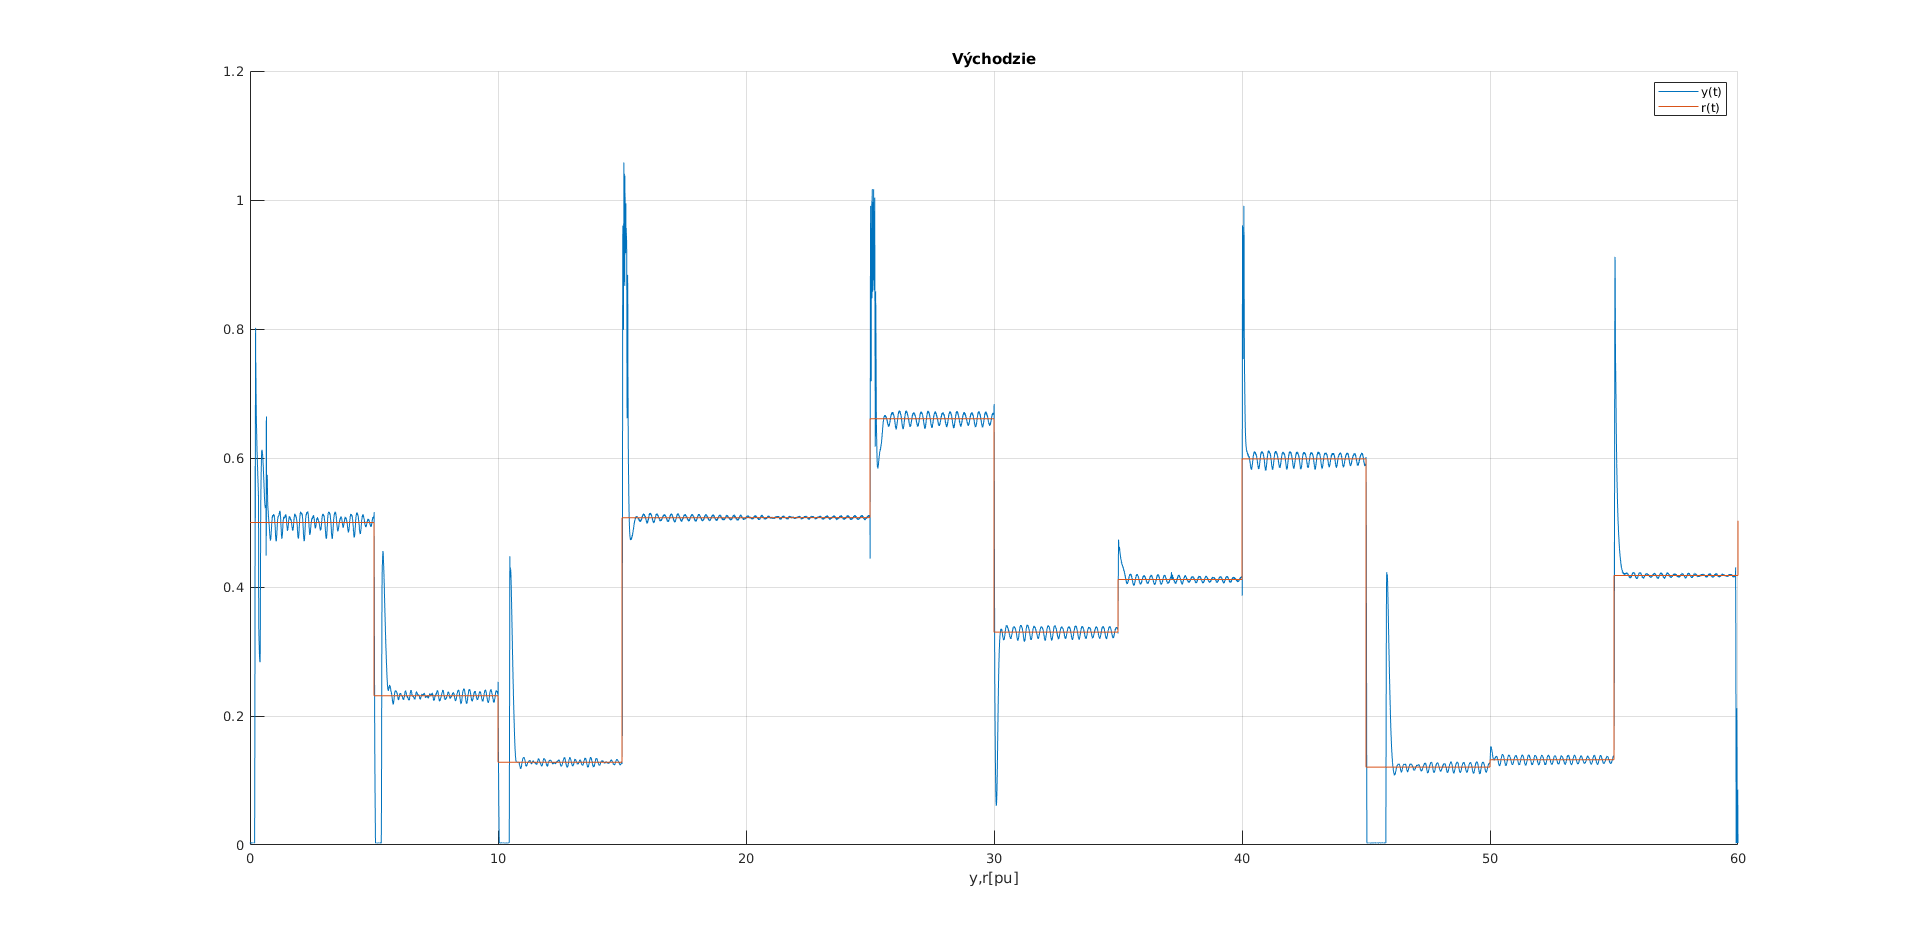
\includegraphics[width=0.8\textwidth]{./include/m4.png}
	\end{center}
	\caption{Graf tretieho merania.}
	\label{fig:meranie3}
\end{figure}

\clearpage

\subsection{Meranie 4}
\label{sec:meranie4}

\begin{table}[!htbp]
	\caption{Koeficienty PID regulatora}
	\label{tab:t4}
	\begin{center}
		\begin{tabular}[c]{|l|l|}
			\hline
			P & 1 \\
			I & 3.2 \\
			D & 0.016 \\
			\hline
		\end{tabular}
	\end{center}
\end{table}

\begin{figure}[!htbp]
	\begin{center}
		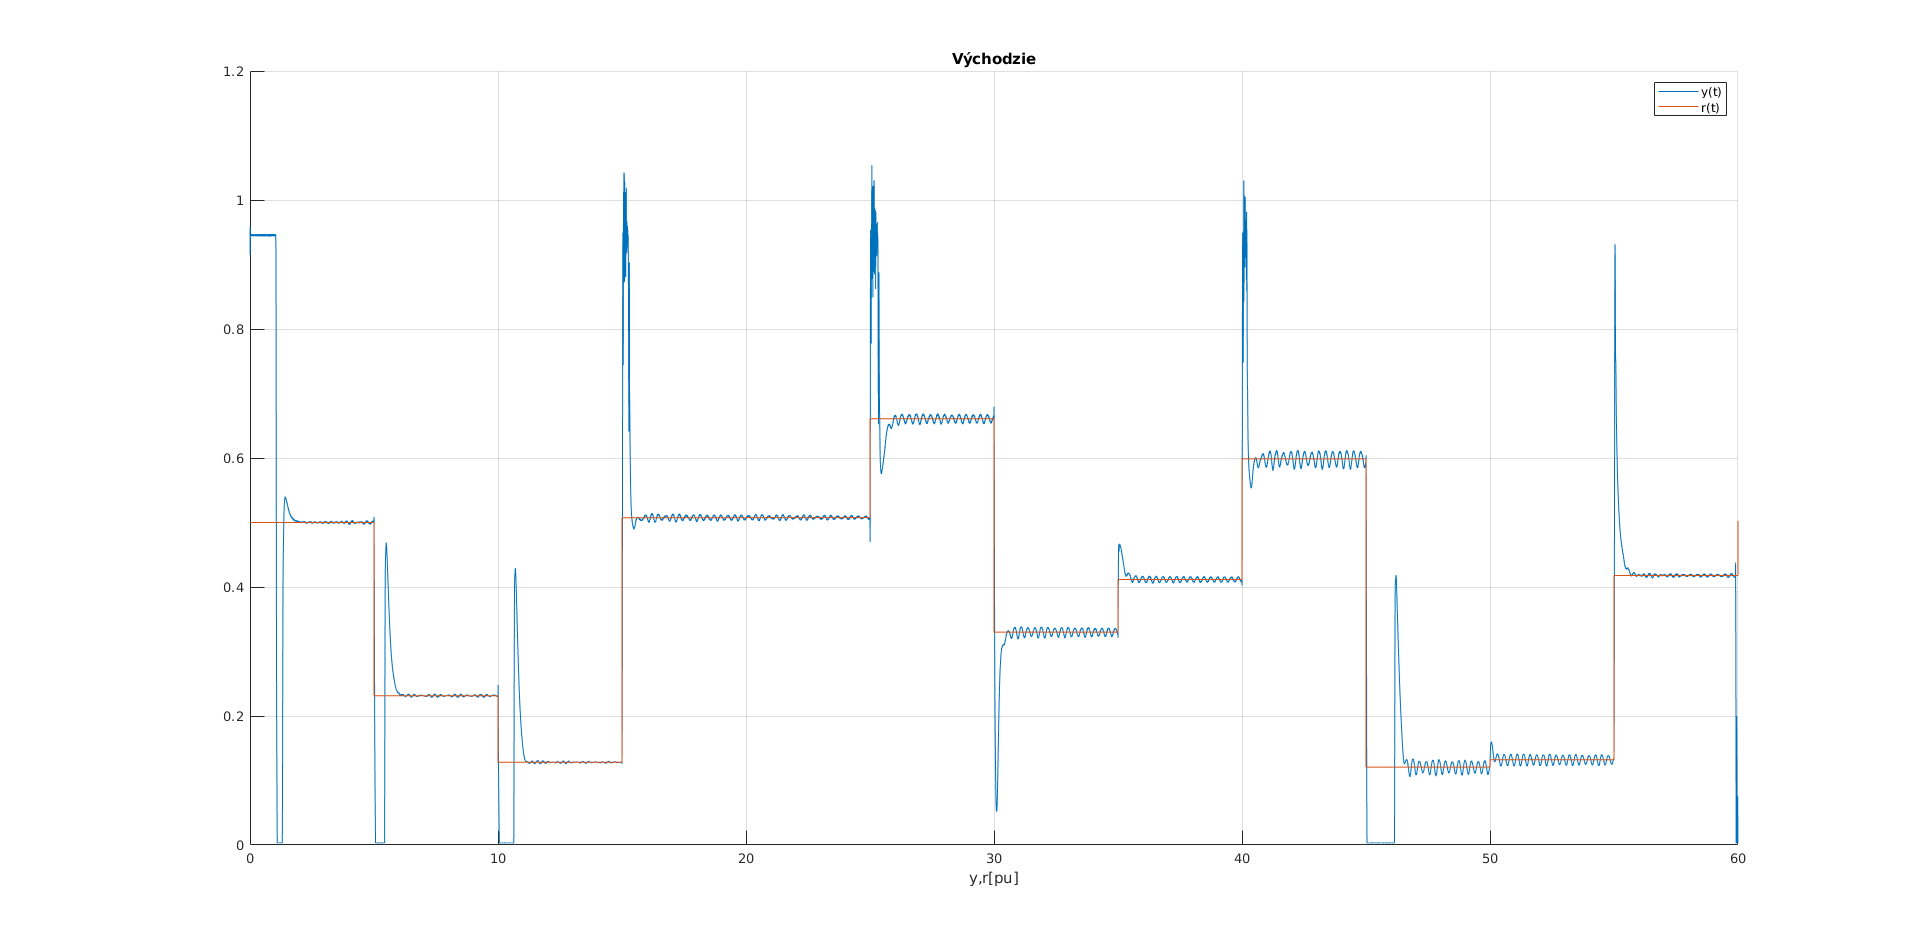
\includegraphics[width=0.8\textwidth]{./include/m6.png}
	\end{center}
	\caption{Graf stvrteho merania.}
	\label{fig:meranie4}
\end{figure}

\clearpage

\subsection{Meranie 5}
\label{sec:meranie5}

\begin{table}[!htbp]
	\caption{Koeficienty PID regulatora}
	\label{tab:t5}
	\begin{center}
		\begin{tabular}[c]{|l|l|}
			\hline
			P & 1 \\
			I & 4 \\
			D & 0.0128 \\
			\hline
		\end{tabular}
	\end{center}
\end{table}

\begin{figure}[!htbp]
	\begin{center}
		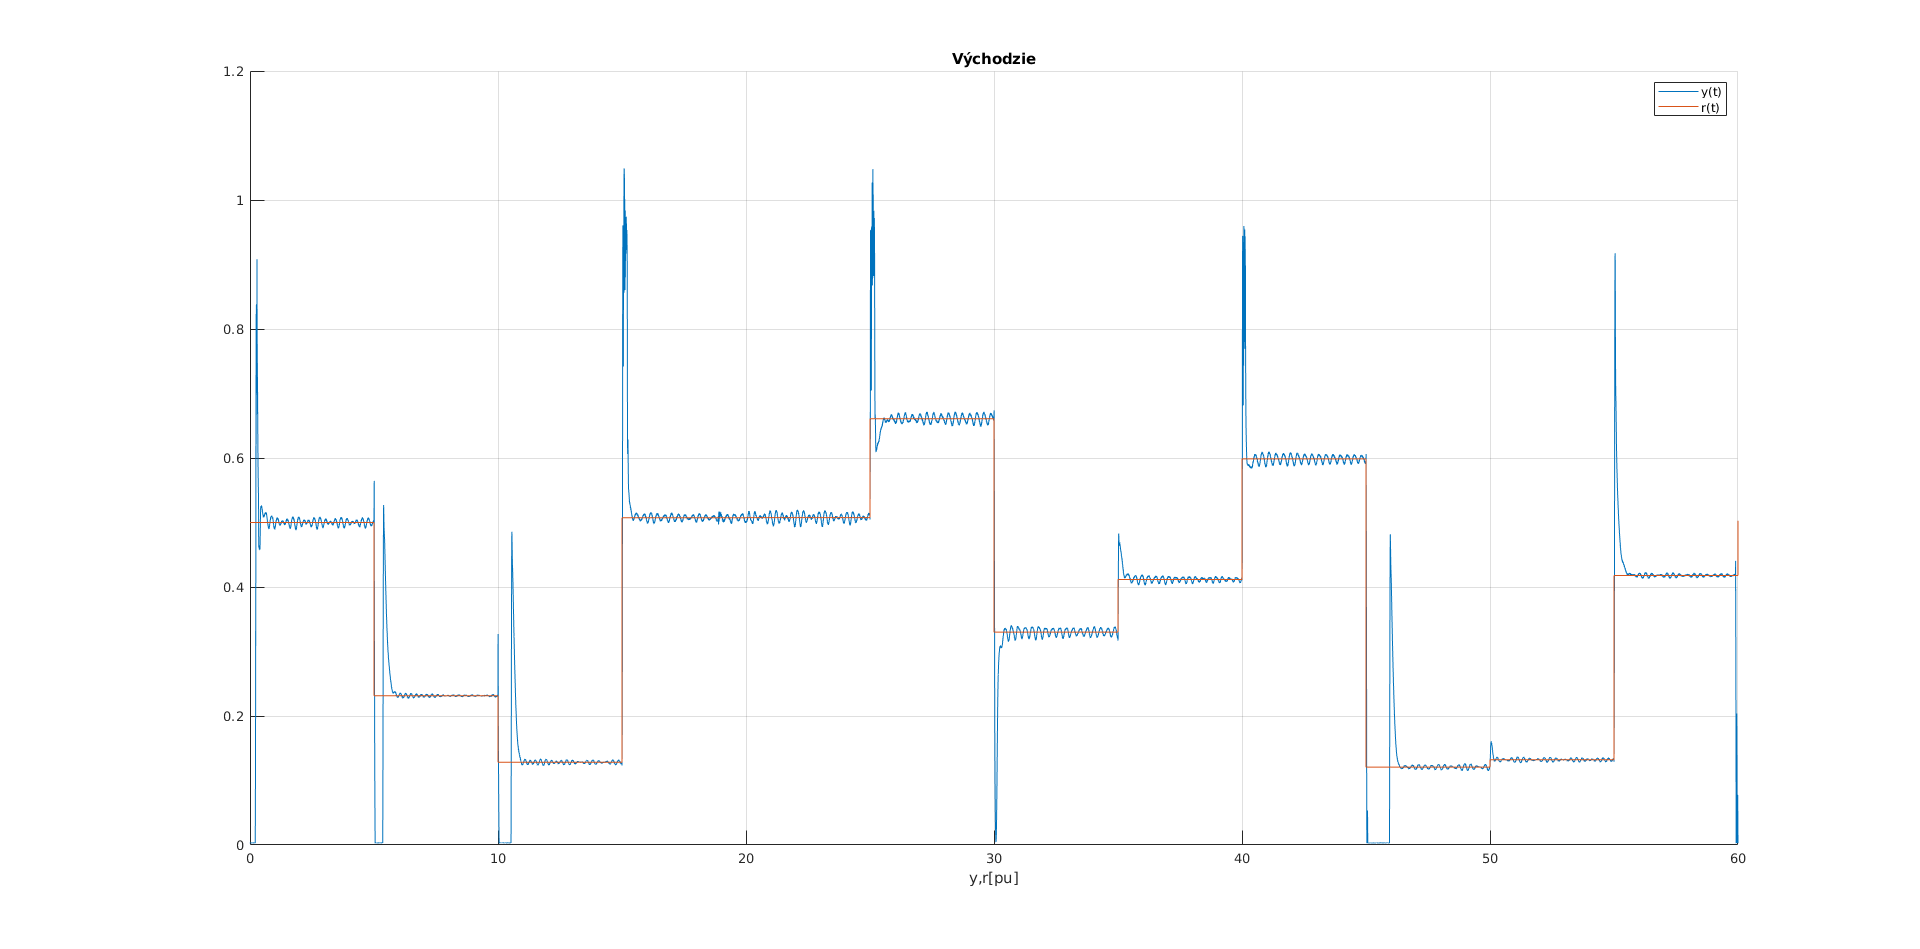
\includegraphics[width=0.8\textwidth]{./include/m5.png}
	\end{center}
	\caption{Graf piateho merania.}
	\label{fig:meranie5}
\end{figure}

\clearpage

\subsection{Meranie 6}
\label{sec:meranie6}


Posledne meranie sa zaobera skumanim vplyvu zvacsenia derivacnej zlozky PID regulatora na~ovladanie magnetickej levitacie.


\begin{table}[!htbp]
	\caption{Koeficienty PID regulatora}
	\label{tab:t6}
	\begin{center}
		\begin{tabular}[c]{|l|l|}
			\hline
			P & 1 \\
			I & 4 \\
			D & 0.0192 \\
			\hline
		\end{tabular}
	\end{center}
\end{table}

\begin{figure}[!htbp]
	\begin{center}
		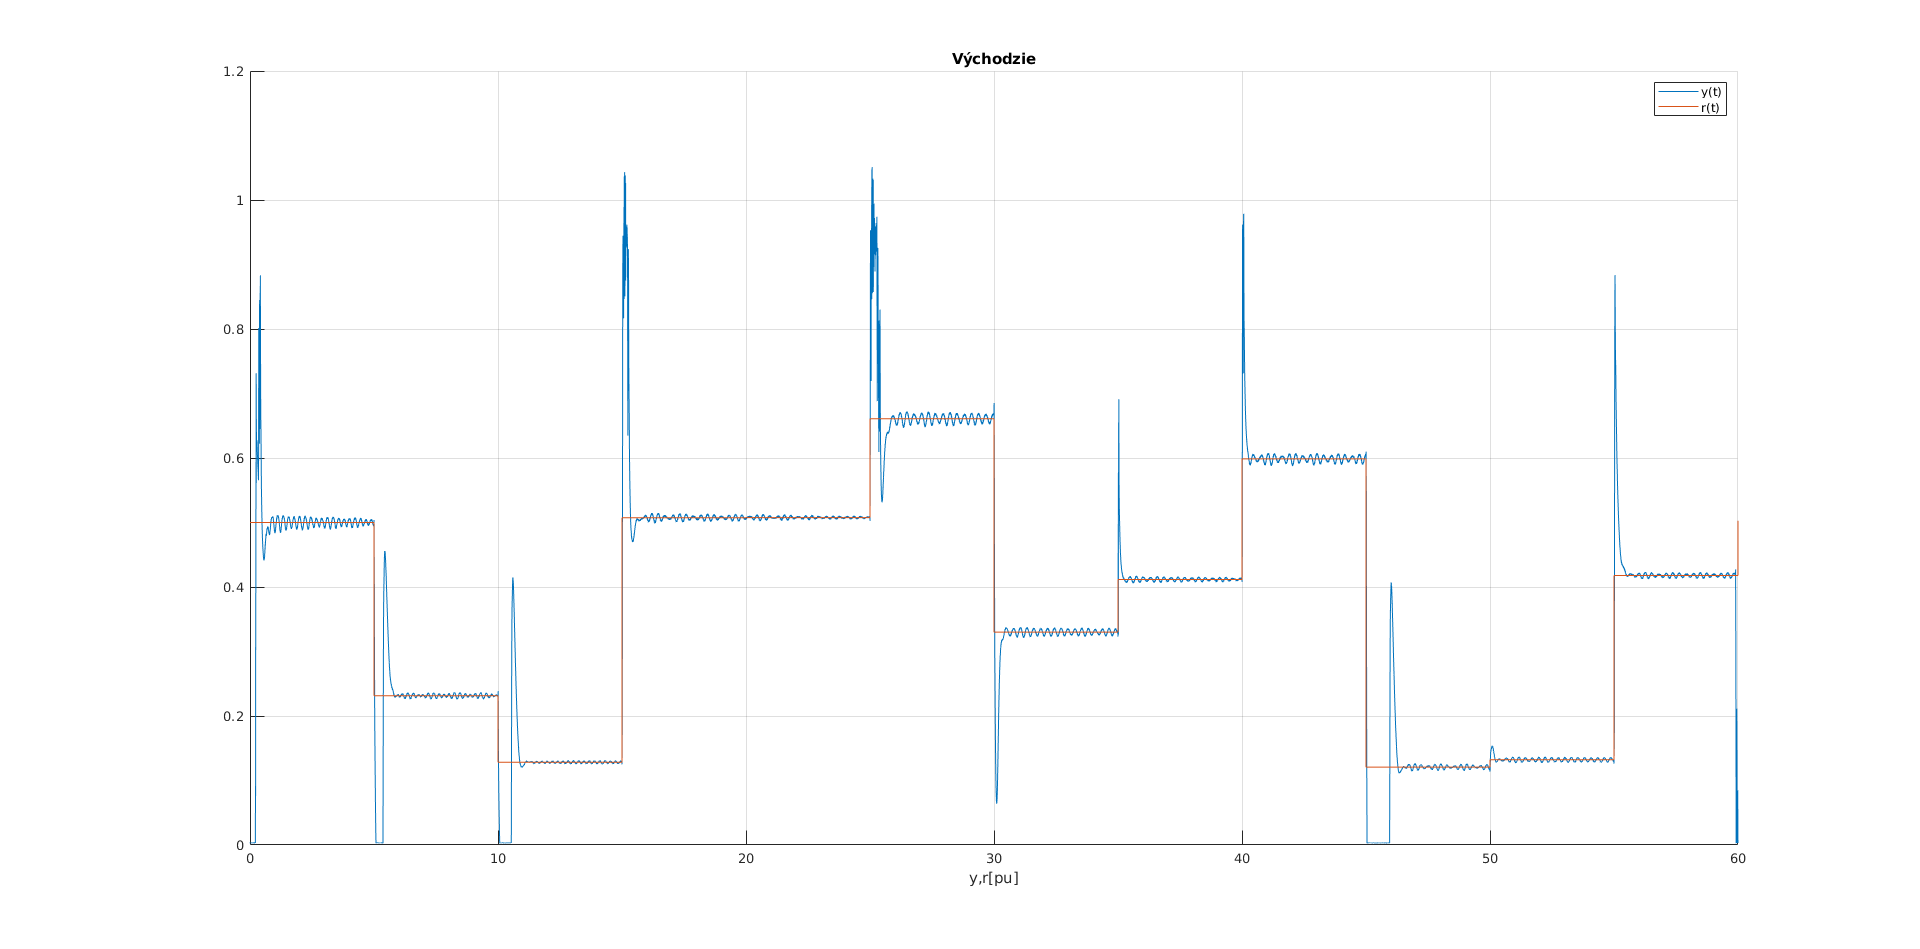
\includegraphics[width=0.8\textwidth]{./include/m7.png}
	\end{center}
	\caption{Graf siesteho merania.}
	\label{fig:meranie6}
\end{figure}

\end{document}

